\begin{figure}[!h]
\centering
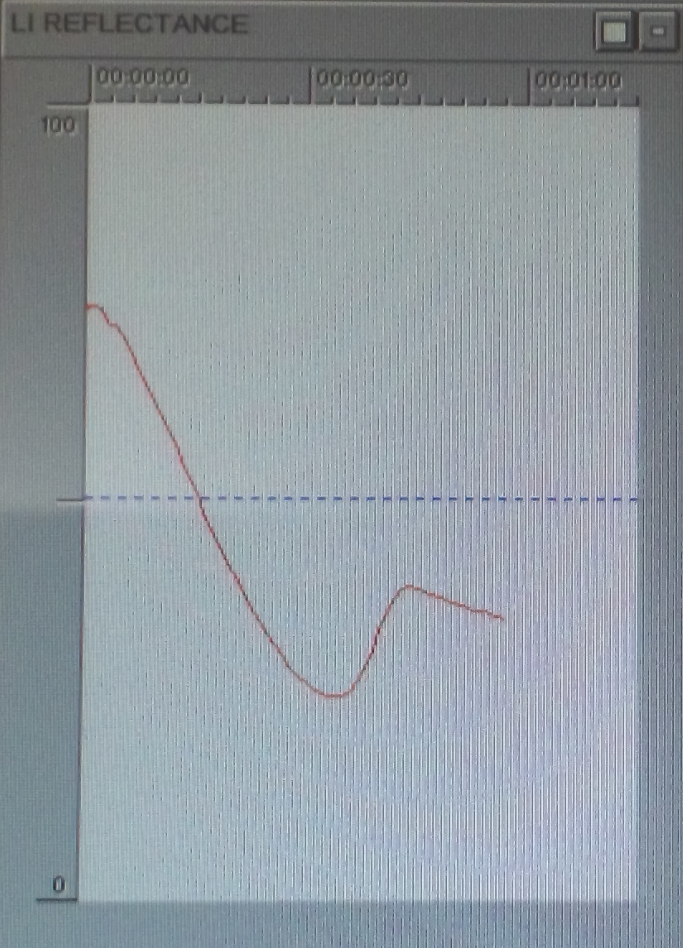
\includegraphics[width=14cm]{figures/oxford_MoSi_etch.png}
\caption{\label{fig:oxford_MoSi_etch}Typical endpoint signal of MoSi etch. The small peak after the dip is interpreted as the end of the etch. Overetch by 10\,s-20\,s after that peak.}
\end{figure}

\begin{itemize}
\item Ash 5\,min
\item Deposit MoSi in AJA
\item Recipe: MoSi \_ jms
\begin{itemize}
\item RF plasma clean for 150\,s at 80\,W
\item Typical DC voltage: 100\,V
\item Deposit MoSi: 50\,s
\item Voltage: 460\,V
\item Current: 440\,mA
\item Deposit a-Si: 66\,s
\item Voltage: 183\,V
\end{itemize}
\item Pattern
\begin{itemize}
\item Spin: SPR600 @ 3000\,rpm
\item Expose: 220\,mJ/cm$^2$
\item Develop: double puddle, 30\,s, 30\,s
\item Run through spin rinse dry
\item Inspect with microscope
\item Etch with Oxford Fl
\begin{itemize}
\item Recipe: opto-WSi-v2-lowHeForCarrier
\begin{itemize}
\item SF$_6$: 1\,sccm
\item Ar: 80\,sccm
\item RF: strike at 30\,W, cut to 10\,W as quickly as possible
\item ICP: 600\,W
\item Pressure: 10\,mTorr
\item He: 5\,Torr
\item Rate: $\sim$\,8\,nm/min
%\item Note: 
\end{itemize}
\item Etch: $\sim$60\,s-70\,s
\item DC bias: 67\,V
\item Use endpoint; typical signal shown in Fig.\,\ref{fig:oxford_MoSi_etch}
\item Insert picture of endpoint signal and log book entry
\end{itemize}
\item Ash: 2\,min
\item Clean: acetone dirty 2\,min, acetone clean 2\,min, IPA, spin rinse dry
\item Inspect with microscope
\end{itemize}
\end{itemize}